\documentclass{article}

\usepackage{geometry}
\usepackage{makecell}
\usepackage{array}
\usepackage{multicol}
\usepackage{setspace}
\usepackage{changepage}
\usepackage{booktabs}
\usepackage{wrapfig}
\usepackage{graphicx}
\newcolumntype{?}{!{\vrule width 1pt}}
\renewcommand\theadalign{tl}
\setstretch{1.10}
\setlength{\parindent}{0pt}
\graphicspath{ {./Images/} }

\geometry{top=12mm, left=1cm, right=2cm}
\title{22S GSB.02005UB Grundprobleme der alten Geschichte}
\author{Andreas Hofer}

\begin{document}
	\section{Einführung - 03.03.2022}
	\section{Der Alte Orient - 10.03.2022}
	Der geographische Raum des alten Orients umfasst drei größere Gebiete, in welchem sich die Teile abspielen:
	\begin{itemize}
		\item{Das Zweistromland zwischen Euphrat und Tigris. Mesopotamien heißt Land zwischen den Zwei Flüssen}
		\item{Das Nilland und das alte Pharaonenreich. Dies wird auch durch die Ägyptologie vertreten}
		\item{Das Gebiet der heutigen Türkei. Im wissenschaftlichen Bereich wird es auch \textbf{Kleinasien} genannt.}	
	\end{itemize}
	In Einheit 3 wird auch noch die Ägäiswelt der Minoischen und Mykonischen Kultur besprochen. \\
	Vom Skript ausgehend wird der Prüfungsrelevante Stoff auf die Zeit bis zum ausgehenden 2. Jahrtausend vor Christus beschränkt. \\
	Die Kapitel 6, 7 und 8 über Neuassyrisches Reich, Achämenidenreich und Spätzeit von Ägypten wird in einem späteren Zeutpunkt behandelt. \\
	\subsection{Mesopotamien}
	Die geographischen Vorraussetzungen Mesopotamiens sind außergewöhnlich besonders, da das fruchtbare Schwemmgebiet der beiden Flüsse zur Entstehung der ersten Hochkultur geführt hat. \\
	Diese fruchtbaren Böden waren in dieser Region besonders wichtig, da es in einem recht niederschlagsarmen Gebiet liegt. Das führt auch heute noch zu großen Geopolitischen Problemen, welche den Wasserreichtum der Flüsse kontrollieren wollen. Diese Machtdynamik ist auch in Ägypten vorhanden. \\
	Im Gegensatz zum landwirtschaftlichen Reichtum in der Region ist es sehr arm an Bodenschätzen, wodurch der Handel in der Region stark ausgeprägt war. \\
	Diese Umstände führten zu einer sehr frühen Urbanisierung in dieser Region. Zusätzlich existierten auch oft Stadtstaateb, mit ausgeprägter Aristokratie. Dadurch wurde die Rivalität zwischen den Städten angefacht, was wahrscheinlich zu einer beschleunigten Wissenschaftsaneignung geführt hat. \\
	Einer der größten Stadtstaaten war die Stadt von \textbf{Uruk} und stellt den ersten Höhepunkt der Machtausdehnung dieses Gebiets da. Dieser Höhepunkt fand im dritten Jahrtausend vor Christus statt. \\
	Eine wichtige Entwicklung in dieser Zeit war die Einführung der Keilschrift, welche schon ab dem 4. Jahrtausend verwendet wurde. \\
	Diese Schrift wurde von mehreren Sprachen verwendet und ist nicht nur auf eine Sprache bezogen. Die Schrift war größtenteils als Verwaltungssprache verwendet um Sachen zu katalogisieren. Trotzdem gab es schon eine literarische Verwendung dessen. Dies war jedoch mehr Propagandaschrift und zur Machtfestigung gedacht, als für Prosa oder Lyriktexte, welche zu diesem Zeitpunkt noch nicht existierte. \\
	Uruks Dominanz wich im frühen 3. Jt. für eine polyzentrische Struktur, in welcher mehrere Städte eine eigene Position einnahmen, jedoch immer noch in Konkurrenz standen. \\
	Es ist emblematisch für Geschichte Macht zu zentralisieren und es gibt stets Beispiele, in welcher Staaten oder Stadtstaaten in der Lage waren ein Gebiet zu beherrschen. \\
	Das zweite größere Reich ist das Reicht von \textbf{Akkad} welches ab etwa 2340 in der Region dominierte. Diese Dominanz bestand für nahezu 200 Jahre. Akkad vergrößerte sein Reich jedoch in den Norden bis in das heutige Syrien. Die Ausdehnung führt in den Norden bis nach \textbf{Subartu} bis \textbf{Elam} in den Osten. Diese Expansion fand unter dem Herrscher Sargon statt, welcher ein weit größeres Heer von bis zu 5000 Mann hielt. \\
	200 Jahre mag in Antiken Maßstäben nicht wie viel wirken, ist jedoch für moderne Verhältnisse eine recht lange Zeit. \\
	Das dritte große Reich war das Reich von \textbf{Ur III}. III steht für die dritte Dynastie von Ur.\footnote{f.d steht für Frühdynastisch} \\
	Ur III fand seine größte Ausbreitung um etwa 2000 v. Chr. und ungefähr 100 Jahre anhielt. \\
	Das letzte große Reich dieser Region war das Reich von \textbf{Babylon}, welches kurz nach Niedergang des Reiches von Ur seinen Höhepunkt fand. Babylon hatte eine ähnliche Ausdehnung wie das Reich von Akkad seinerzeit. Diese Ausdehnung geschah wiederum unter dem Herrscher \textbf{Hammurabi} von Babylon. Hammurabi ist zudem für eine Einführung der Keilschrift als kulturelles Gut verwantwortlich. Die \textbf{Stele von Hammurabi} ist eine 2 Meter große Stele, ausgestellt im Louvre, welche einen Teil des Codex von Hammurabi darstellt. Der Codex von Hammurabi und andere gefundene Texte zeugen von einem ausgeprägten Rechtstext, was ein Indiz einer Hochkultur ist. \\
	Die Keilschrift auf der Stele ist ansatzweise erahnbar und die unterschiedlichen Rechtsteile, welche man finden kann beinhalten das:
	\begin{itemize}
		\item{Liegenschaftsrecht}
		\item{Schuldrecht}
		\item{Erbrecht}
		\item{Sklavenrecht}
		\item{Eherecht}
	\end{itemize}

	Das Babylonische Reich von Hammurabi bestand von 1790 v.Chr. bis 52 v.Chr. und stellt das längstwährende Reich der Region da. Obwohl spätere Herrscher schwächer waren als Hammurabi selbst, konnte es sich einige Zeit etablieren. \\
	Babylon wurde letztendlich von den Hethitern aus der heutigen Turkei erobert. \\
	Die Religion stellte in dem Gebiet auch immer wieder die Legitimation der Herrscher da. \\
	Durch die Verwaltungsschrift innerhalb der Stadtstaaten führte auch zu einem ausgeprägten Beamtenapparat, welcher später auch in Ägypten eine wichtige Rolle spielte. \\
	Durch die Übernahme Babylons nahm das \textbf{Hethitische Reich} eine Vormachtstellung ein und dehnte sich bis in das heutige Kairo aus. \\
	Zu dieser Zeit baute das Reich auch die Hauptstadt \textbf{Hattu[[ADD s with thingy]]a} signifikant aus. \\
	Die Hethiter führten auch mehrer kriegierische Auseinandersetzung mit den antiken Pharaohnen um ihre Macht auszudehnen. \\
	Bei den Hethitern war es jedoch wiederum lediglich eine militärische Expansion, wodurch auch die Herrscherposition und Legitimation von der Expansion abhängig wurde. \\
	Im Gegensatz zu den Babylonern, wo der Herrscher durch eine Aristokratie gestützt wird, war im Hethitischen Reich der Herrscher selbst viel mächtiger. \\
	Ebenfalls hatte die Gemahlin des Hethiterherrschers eine ausgeprägte Funktion, wodurch sie selbst in der Lage war Verträge mit anderen Nationen zu unterzeichnen. \\
	\subsection{Ägyptisches Reich}
	Ägypten, obwohl als Territorialstaat angenommen, ist und war früher auch fast nur das Reich des Nils, also die Bevölkerung begrenzte sich fast ausschließlich auf die Gebiete unmittelbar um den Nil. \\
	Die Griechen bezeichneten die Ägypter als Geschenk des Nils, obwohl sie nicht wussten woher die Überschwemmung des Nils stammt. Diese bracht stets Nährstoffe und Sedimentgestein mit sich, was das Schwemmland sehr fruchtbar machte. \\
	Der Umstand, dass das Ägyptische Reich von Wüste umgeben war, war auch eine hevorragende Verteidigung gegenüber einfallender Mächte, da jede Armee zuerst die Wüste durchqueren musste, und die meisten Herrscher ihre Armeen gar nicht über einen solchen Zeitruam ernähren konnten. \\
	Das Ägyptische Reich wurde über seine lange Geschichte trotzdem öfters erobert:
	\begin{itemize}
		\item{Zuerst durch das Persische Reich}
		\item{Durch die Griechen unter Alexander dem Großen}
		\item{Durch die Römer}
		\item{Durch Moslemische Mächte}
	\end{itemize}

	Ägypten kann in drei Zeitabschnitte geggliedert werden:
	\begin{itemize}
		\item{Das Alte Reich: 2650 - 2160 v.Chr.}
		\item{Das Mittlere Reich: 2025 - 1650 v.Chr.}
		\item{Das Neue Reich: 1550 - 1070 v. Chr.}
	\end{itemize}

	Zusätzlich gab es zwischen den beiden ersten Dynastien jeweils zwei Zwischenzeiten, in welcher keine größere Macht eine Prägung hatte. Ebenfalls wird nach dem Neuen Reich die Spätzeit definiert, welche von 1070 - 525 v. Chr. dauerte. Zu dieser Zeit gab es einige schwächere Pharaohnen, welche über Ägypten herrschten. \\
	
	Ungefähr zur selben Zeit als die Keilschrift in Mesopotamien enstand (Die Keilschrift wird als etwas älter angesehen), fand auch die Ägyptische Schrift ihren Ursprung. Für lange Zeit galt das Ägyptische als nicht lesbar, jedoch wurde während der Zeit Napoleons der \textbf{Stein von Rosetta} gefunden, welcher in Ägyptisch sowie Altgriechisch geschrieben war. Nach etwa 20 Jahren, im Jahre 1822, wurde das Ägyptische schließlich vollständig entziffert und brachte das Fach der Ägyptologie hervor. Ebenfalls führte es zu einem Boom des Interesses in der westlichen Elite für die Ägyptische Zeit. \\
	
	Die staatliche Ordnung in Ägypten wurde bereits sehr früh durch den Pharaoh geprägt, welcher der Herrscher und Eigentümer des Landes ist. Unter diesem Pharaoh war das Reich geeint. Der Pharaoh hatte, nach heutigen Maßstäben, eine absolutistische Macht und wurde durch Erbfolge geregelt. Später war der Pharaoh auch durch Gott gesandt und erhielt so seine Legitimation. \\
	Dies wurde durch die zentrale Religion des Reiches ermöglicht, welcher ein wichtiger Teil der Gesellschaft war. \\
	Der Staat ist sehr zentralistisch organisiert um einiges strikter als es im Hethitischen Reich der Fall war. Die Befehlskette war hierarchisch von oben nach unten geregelt, wodurch ein gemeiner Bürger praktisch keinen Einfluss auf die Geschehen hatte. \\
	Jeder Abschnitt des Landes war in Gaue gegliedert, welcher durch einen Statthalter verwaltet wurde und wieder seinen eigenen Verwaltungssitz hatte. \\
	Ebenfalls war die Besteuerung der Bevölkerung ein zentraler Bestandteil des Reiches. Die Steuern waren stets an die höhere soziale Position abzugeben und von dort weiter verteilt. \\
	Die Legitimation dieses Machtapparats und Rechtfertigung für Steuern war die Sicherheit und Rechtsordnung innerhalb der Region. Dies war einerseits durch die Religion, aber auch durch die militärische Macht gewährt. \\
	Wirtschaftlich war Ägypten außerordentlich effektiv, was durch die Konstruktion der Pyramiden ersichtlich wird, welche ein enormer menschlicher und wirtschaftlicher Aufwand waren. Die Pyramiden waren gigantische Grabbauten, wobei die Cheops-Pyramide einen Grundriss von 200x200 Meter maß und 150 Meter hoch war. \\
	Das Ende des Alten Reiches wurde durch eine wachsende Macht der regionalen Eliten eingeleitet, was wiederum den Pharaoh schwächte. Schließlich kam es mit dem mittleren Reich zu einer neuen zentralen Machtstruktur. \\
	Die zweite Zwischenzeit war wiederum durch Machteinflussnahme von außen geprägt, in welcher das Reich der Hyksos über Ägypten herrschte. Mit dem Neuen Reich kam es jedoch schließlich wieder unter eigene Kontrolle. \\
	
	Im Neuen Reich von Ägypten konnte nicht nur die Macht im eigenen Reich gefestigt werden, sondern versuchte diese Macht auch nach außen zu projezieren. Diese Projektion äußerte sich in Kämpfen zwischen den Hethitern, aber auch den Babylonieren und den Griechen. \\
	Was hinzugefügt werden sollte ist, dass, obwohl ein Pharaoh ein absoluter Herrscher war, dieser nicht unbedingt eine Stärke im Reich gezeigt hat. Diese wurden oft durch die Aristokratie alsbald entledigt. Ein solches Beispiel ist \textbf{Tutenchamun}, dessen Grab ungeöffnet war. \\
	Nach Ende des Neuen Reichs findet langsam ein Zusammenbruch des intranationalen Machtsystems statt, welcher durch die Ägäis ausgeht und eine langfristige Schwächung der Herrscher dieses Gebiets führt. Von dieser Zeit aus sind nicht nur in Ägypten sondern auch im Zweistromland Gebiete oft durch fremde Herrscher besetzt, anstatt Selbstbestimmung zu haben.

	\section{Wirtschaft im Alten Orient und frühe Ägäis - 17.03.2022}
	\subsection{Wirtschaft: Mesopotamien und Ägypten}

	Die Wirtschaft in Mesopotamien war zwar nicht so trocken wie in Ägypten, hatte jedoch eine ausgeprägte Wasserwirtschaft und führte oft zu Stadtstaaten die sich an einem der Flüsse ansiedelt. Mesopotamien war eine \textbf{Redistributionswirtschaft}, was bedeutet, dass der Boden zum Großteil im Besitz des Stadtstaates, also dem Herrscher und der Aristokratie, liegt und die gemeine Bevölkerung diesen verwenden kann, aber diese auch zu Kriegs- und Bauzwecken herangezogen werden konnte. Gleichzeitig wurde die Bevölkerung jedoch für diese Dienste wiederum mit Waren entlohnt, woher der Name rührt. \\
	
	Die Wirtschaft in Mesopotamien beruhte noch nicht auf einer Währung sondern rein auf Warentausch, weshalb auch oft der Wert von waren untereinander abgewogen wurden, also wie viel eine Länge Leinen im Vergleich zu Weizen wert war. Für Rohstoffe musste jedoch, wie zuletzt besprochen, mit anderen Völkern getauscht werden, was auch einen regen Handel in der Region ankurbelte. \\ \\
	
	In Ägypten gab es eine größtenteils ähnliche Situation wie in Mesopotamien. Ägypten ist zuallererst das Land am Nil, obwohl oft der gesamte Saharateil auch mitgezählt wird, jedoch gibt es einen scharfen Schnitt zwischen fruchtbarem Land und trockener Wüste. Die Bewässerung war ein Grundpfeiler der altägyptischen Gesellschaft. Dies geschah zuerst durch die natürliche Überflutungszeit des Nils, aber später auch durch eigens angebaute Kanäle, welche das Wasser weiter verbreiten. Die Nilschwemme rührt von den Monsunwinden, welche extrem viel Wasser in die Afrikaregion einführen, was wiederum um das Einzugsgebiet vom Nil abregnet und zu dieser jährlichen Überflutung führt. Während dies heute bekannt ist, wurde es im antiken Ägypten als "Geschenk des Nils" angesehen. \\
	Zurück zur Wirtschaft: Auch in Ägypten gab es eine ähnlich funktionierende Redistributionswirtschaft, wo Bauern fremdes Land bewirtschaften und einen Teil davon abgeben und hierfür auch anderes wie Baumaterialien erhalten. Während es ähnlich von Mesopotamien war, war es ungleich größer als das Zweistromland, was die Administration komplexer werden ließ. \\
	Rohstoffmäßig war Ägypten besser gestellt als Mesopotamien und war nicht abhängig vom Handel um essentielle Ressourcen zu erhalten. Trotzdem wurde reger Handel, vor allem mit dem nubischen Reich, getrieben, größtenteils um Waren zu erhalten, welche in Ägypten nicht erhätlich waren (Größtenteils Gold). \\
	
	\subsection{Frühe Ägäis}
	Während aus Sicht der Hethiter und Ägypter die Ägäis zuerst eher als Randregion angesehen wurde, gewann das heutige Griechenland mehr Einfluss. Kleinere Zentren innerhalb der Region dominieren mit der Zeit immer mehr und bringen auch bald selbst Kulturen hervor. Zu dem Zeitpunkt wurde Bronze als Metall angesehen, welches lange Zeit dominant war. Es folgte auf die Kupferzeit, was jedoch eher als Randnotiz angesehen wird, da diese nicht so lange währte. Während Kupfer ein Metall ist, ist Bronze eine Legierung aus Zinn und Kupfer. Dies verlangt einige Sachen um zu funktionieren, da man Vorkommen beider Metalle, sowie Möglichkeiten diese zu legieren und bearbeiten benötigt. Dies zeugt viel mehr von einer Hochkultur im Vergleich zur Verwendung von bloßem Stein oder Kupfer. \\
	Die Bronzezeit im Ägäisbereich ist in drei Teile geteilt:
	\begin{itemize}
		\item{Frühe Bronzezeit - 3100 - 2100 (FK, FH, FM)}
		\item{Mittlere Bronzezeit - 2100 - 1700 (MK, MH, MM)}
		\item{Späte Bronzezeit - 1700 - 1100 (SK, SH, SM)}
	\end{itemize}
	Gleichzeitig wird es in drei geographische Gliederungen:
	\begin{itemize}
		\item{Kykladen/Kykladikum}
		\item{Festland/Helladikum}
		\item{Kreta/Minoikum}
	\end{itemize}
	Diese werden wieder in Früh-, Mittel-, Spätzeiten aufgeteilt: Frühes Kykladikum, Mittleres Kykladikum und Spätes Kykladikum etc. \\
	Wenn man diese Zeitspannen mit den Zeiten von Mesopotamien und Ägypten vergleicht, sieht man, dass diese zwar etwas früher beginnen, jedoch im Endeffekt um 1100 konvergieren. \\
	Während Hieroglyphen in Ägypten zu einer umfassenden Datierung geführt haben, ist das in der Ägäis nicht so genau zu datieren, weshalb die meisten der Zeiten grobe Schätzungen sind. \\ \\
	
	Zusätzlich ist in der Ägäis die Art der Quellensuche eine sehr unterschiedliche wie in Mesopotamien. Unter anderem gibt es in der Ägäischen Frühzeit schriftliche Quellen, sogenannte \textbf{Linear A und B Tafeln}, wovon Erstere jedoch noch nicht entschlüsselt worden sind. Zusätzlich gibt es viele archäologische Quellen. Besonders in der Keramik konnte man anhand der Art der Herstellung oder der Zusammensetzung selbst, genaue Entwicklungen feststellen. \\
	Die erste erwähnenswürdige Stadt ist \textbf{Troja}, welches im Vergleich zu den drei Kulturen etwas außenvor steht. Jedoch ist es aufgrund der intensiven Ausgrabungen, welche in dem Gebiet durchgeführt wurden, ein Paradebeispiel der griechischen Archäologie. Vor 150 Jahren wurden bereits die Ausgrbaungsstätten gefunden, welche auf Troja Rückschluss gaben. Während es der Ort der Lyrik von Homer war, hat dieser jedoch auch eher im Retrospekt geschrieben, weshalb diese wahrscheinlich nicht geographisch akkurat sind. \\
	In Troja konnte man die Bildung der Siedlung in außerordentlichem Detail rekonstruieren. Diese werden als Phase I bis Phase IX bezeichnet. Um 3000 in Phase I gab es zwar nur einige Hütten, hatte jedoch bereits eine Verteidigungsmauer. In Phase II gibt es eindeutige panmäßige Erweiterungen, mit Terrassierungen und Umfassungsmauern. In Phase III ist Troja deutlich weniger dicht besiedelt, wahrscheinlich durch Zerstörungen, welche nur langsam wiederaufgebaut wurden. In Phase IV hat sich dort eine andere Bevölkerungsgruppe angesiedelt, mit Zuwanderern aus Anatolien und die Stadt langsam wieder aufgebaut wird. In Phase V ist ein deutlicher Aufschwung erkennbar, wahrscheinlich angeregt durch Handel mit Kreta und anderen Kulturen. Jedoch wird zum Ende auch ein Verlassen der Stadt erkenntlich, was jedoch nicht auf Zerstörungen zurückführen ist, sondern wahrscheinlich eher auf Krankheiten. In Phase VI wird Troja erneut durch eine neue Bevölkerungsgruppe besiedelt, diesmal [[Nubiern]] und markiert die Blütezeit der Stadt. Zu dieser Zeit nimmt Troja einen Knotenpunkt ein, da es für den Nord-Süd Verkehr essentiell war. Dies rührte daher, dass bei der Fahrt nach Süden oft Nordwinde herrschen und man diesen abwarten muss um weiterfahren zu können. In dieser Phase kommen auch immer wieder Brände vor, was jedoch nicht zu einem Verlassen führt. In Phase VII sind größere Brandkatastrophen nachweisbar und auch die Besiedelung einer weiteren Bevölkerungsgruppe wird nachgewiesen : Luwier. In Troja wurde zuerst recht grob vorgegangen, da man nocht nicht genau über diese Vorgänge Bescheid wusste, bzw. welchen Schaden dieser verursacht. Der \textit{Schliemann-Graben}, welcher in Troja gegraben wurde, ist in der Archäologie noch heute ein Begriff. \\ \\
	
	Um nun wieder auf die Hochkulturen der Ägäis zurückzukommen. Die entscheidenden Epochen der Bronzezeit sind das Mittelminoische und das Späthellenikum, welche auch in größerem Detail besprochen werden. Der Rest wird größtenteils zusammengefasst.\\
	\subsection{Ägäisgebiete:}
	\subsubsection{Frühes Kykladikum}
	Das Frühkykladikum, in den zentralen Inseln Griechenlands, auch als Kykloskreisinseln bezeichnet, gab es kleiner Küstennahe Siedlungen, welche später ins Hinterland übersiedelten und auch stärker befestigt wurden. Man kann hier auch einen Minoischen Einfluss nachweisen, größtenteils durch Handel. Die Wirtschaft war recht rudimentär und bestand größtenteils aus Fischerei und Landwirtschaft. Jedoch ist der Boden in dieser Region eher unfruchtbar, weshalb die Bevölkerungsanzahl begrenzt war. Ein wichtiges Gut der Region ist Obsidian, also Vulkanglas, besonders von der Insel Milos. Dieser wurde oft als Messer verwendet. \\
	\subsubsection{Frühes Minoikum}
	Kreta unterschied sich von den Kykladeninsel, da der Boden bedeutend fruchtbarer war weshalb auch größere Bevölkerungen ernährt werden konnten. Hier lassen sich auch Handelskontakte zu Ägypten und dem Mesopotamischen Raum nachweisen. In Kreta wurde auch eine staatliche und hierarchische Struktur angenommen, welche auf der Ägyptischen basiert, was die Handelsbeziehungen unterstützt. \\
	Später gab es auf Kreta größere Zerstörungen, welche wahrscheinlich auf die Luwier zurückzuführen sind. \\
	\subsubsection{Frühes Helladikum}
	Am Festland Griechenlands waren Siedlungen größtenteils an den Flüssen. Zu diesem Zeitpunkt gab es auch schon Handel mit den Kykladen und den Kreten. Die Grundlage der Wirtschaft ist, wie immer, Landwirtschaft, aber auch Gewerbe da das Festland Griechenlands sehr unterschiedlich ist. Die furchtbarsten Gebiete waren um Mykenes \\
	Die Luwier sind eine Bevölkerungsgruppe aus dem Westasiatischen Raum, welche in Teilen der heutigen Türkei lebten. Diese drängten oft in die Ägäis und beeinflussten diese auch. \\
	\subsubsection{Mittleres Kykladikum}
	In der Mittelbronzezeit werden die Siedlungen in den Kykladen oft wieder zerstört aber auch wieder aufgebaut. Hierdurch entstanden umfangreiche Zentren und Befestigungsanlagen um zu widerstehen. Es gab jedoch auch Handelsbeziehungen zum Festland sowie nach Kreta. Der Einfluss von Kreta ist zu diesem Zeitpunkt bedeutend stärker als noch in der Frühbonzezeit. \\
	\subsubsection{Mittleres Minoikum}
	In Kreta selbst ist ein bedeutendes Bevölkerungswachstum nachweisbar. Ebenfalls wird der Verwaltungsapparat straffer. Hier werden in Teilen Kretas, vor allem in Knossos, große Paläste gebaut, welche als Residenz und Handelszentrum dienten. \\
	In Kreta gab es wiederum wieder eine Redistributionswirtschaft wobei die Paläste als Zentrum agierten. Der Handel mit Ägypten und dem Orient bleibt aufrecht und nimmt sogar bedeutend zu. Gleichzeitig findet jedoch auch eine Kolonialisierung dieser Gebiete statt, wobei Handelsaußenposten gebaut werden. Kreta hatte zu diesem Zeitpunkt etwas, was oft als \textbf{Thalassokratie} bezeichnet wird. Kreta hatte eine umfangreiche Seeherrschaft und übte auch großen Einfluss auf seine Umgebung aus. Später sind größere Zerstörungen auf Kreta nachweisbar, was jedoch eher Naturkatastrophen zuzuschreiben ist. Die Paläste, welche zerstört wurden, werden noch größer und pompöser wiederaufgebaut. Dies wird auch als die \textbf{Neupalastzeit} bezeichnet. Aus dieser Zeit stammen auch die angesprochenen Linear-A Tafeln, welche trotz fehlender Entschlüsselung als Admministrations und Wirtschaftstafeln gesehen werden. \\
	Auf Kreta gab es umfangreiche Palastzentren. Die größten Zentren waren Knossos, Zakros und [[ADD MORE PALACES]]. Die Paläste waren umfangreiche Bauten, welche als Residenz, Handelszentrum und theologischer Ort verwendet wurden. \\
	Zu dieser Zeit war auch die Palastanlage in Zakros aufgrund der guten Lage von großem Einfluss. \\
	\subsubsection{Mittleres Helladikum}
	Während Kreta zu dieser Zeit aufblühte, war das Festland eher durch kleinere Dörfer besiedelt, welche jedoch zahlreicher waren. Hier ist im Vergleich ein Rückgang des Wohlstands zu verzeichnen. \\
	\subsubsection{Spätes Minoikum}
	In der späten Bronzezeit ist dieses Verhältnis jedoch umgekehrt und das Festland dominiert über Kreta. In Kreta dominieren die Paläste zwar lokal, verlieren jedoch im großen an Einfluss, was Knossos zur einzigen größeren Stadt macht. Später sind auf Kreta umfangreiche Plünderungen und Zerstörungen der Paläste nachzuweisen. Das Festland nimmt die Insel Kreta hier komplett ein und ist unter dessen Kontrolle. \\
	\subsubsection{Spätes Helladikum}
	Am Festland gab es unterdessen eine Blütezeit, wobei Mykenes als dominante Stadt etabliert wird, was auch zur Bezeichnung dieser Ära zeugt: Die Mykenische Zeit. \\
	Siedlungen welche von der Bevölkerung der Mykenischen Welt gebaut wurden sind oft viel befestigter und größer ausgebaut, was diese zu einflussreichen Zentren des Handels macht. Aus dieser Zeit stammen die Linear-B Tafeln. Von Mykenes ausgehend übernimmt diese Kultur größtenteils die Ägäis und führt zu einer recht kulturell homogenen Gesellschaft. Diese Einigung führt später dazu, dass Griechenland geeint mit den Hethitern agieren kann. Dies ist aus Schriften der Mykener und Hethiter ersichtlich. Mykenes und das Hethiterreich sind schließlich auch in mehrere Kämpfe verwickelt, während dieses mit den Ägypten kämpft. \\
	Der Niedergang der Mykenischen Welt, welcher auch zu einer Schwächung des Hethiterreichs und Ägypten führt, passiert durch einige Naturkatastrophen in der Umgebung, aber auch durch Auseinandersetzungen zwischen einiger der Paläste in der Ägäis, welche zu Einbußen im landwirtschaftlichen Ertrag führte. In den Linear-B Texten wird dies beschrieben, während jedoch auch von Druck aus dem Norden geschrieben wird. Mit dem Wegfall des Mykenischen Reich fallen für Ägypten wichtige Handelskontakte weg. Das Hethiterreich verschwindet zu dieser Zeit nahezu komplett. Es wird vermutet, dass dies durch Druck aus Nordwesten geschehen war. Die Ägypter sprachen von den "Seevölkern". Welche Völker dies waren ist unersichtlich. Es könnte sein, dass es die Mykener selbst waren, welche aufhörten Handel zu führen. Nach dem Untergang des Mykenischen Reichs wird die Zeit oft als "Dark Ages" der Umgebung bezeichent, da sehr wenig darüber bekannt ist, da es fast keine Hinweise gibt.
	
	\section{Geometrische Zeit und Archaik - 24.03.2022}

	Die Geometrische Zeit ist ein recht archäologischer Begriff. Die Geometrische Zeit (ca. 900-750 v. Chr.) ist nach archäologischen Funden in Athen benannt. Diese Funde hatten sich danach auch auf weitere Zentren in Griechenland ausgeweitet. So gabes weitere Funde aus Korinth, Argos, Boiotien, Euboia und den Kykladen. Die Funde sind Vasen und Skypha mit sehr kantigen Mustern, welche diese geometrischen Formen bilden. Am Anfang der geometrischen Zeit waren die Bemalungen recht spärlich. In späteren Vasen bemerkt man, dass diese schon bedeutend enger gemalt wurden. In der spätgeometrischen Zeit (750 - 700 v. Chr.) ist schließlich die nahezu ganze Vase mit Formen bemalt. Eine der bekanntesten Vasen dieser Zeit ist die Dipylon-Vase. Der Name rührt auch daher, dass ein Großteil des Verständnisses dieser Zeit aus der Archäologie stammt. 
	\begin{figure}
	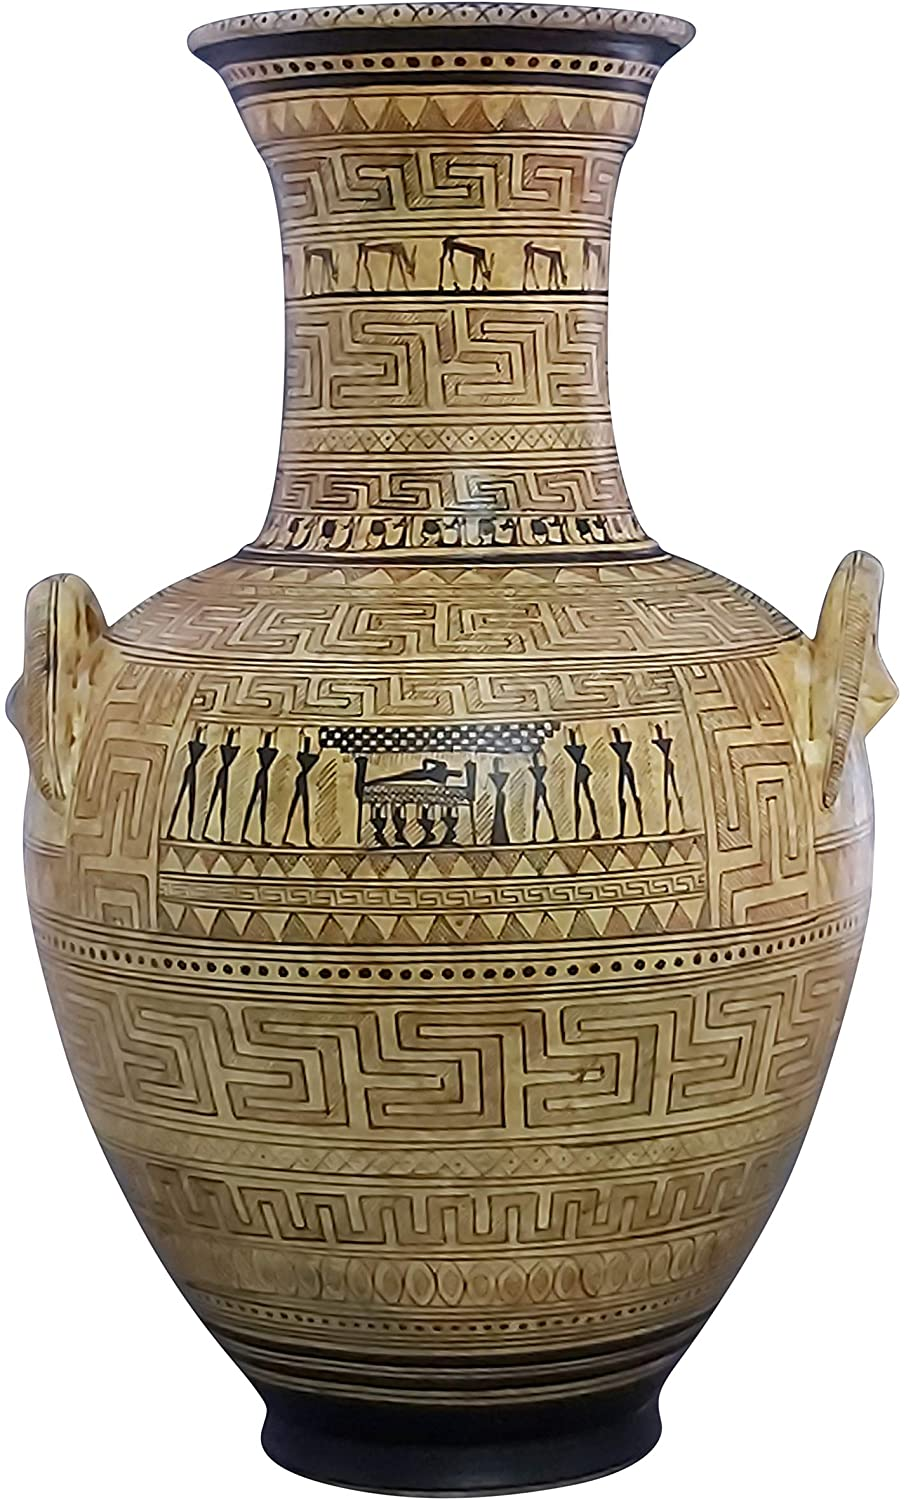
\includegraphics[scale=0.2]{Dipylon.jpg}
	\end{figure}
	Beim Übergang der geometrischen Zeit in die Archaik (600 v. Chr.) ist wiederum eine Änderung der Bemalung, wo eine Entwicklung weg von geometrischen Figuren und mehr zu Personen und Figuren bemerkbar ist.
	\subsection{Das Perserreich}
	Um die Antike zu verstehen, muss man zuerst über das Perserreich reden, da diese ewigen Widersacher der Griechen sind. Persien nahm einen recht bescheidenen Anfang zu 557 a.c. etwas östlich von Mesopotamien nimmt, weitet es sich über die nächsten 18 Jahre bis nach Griechenland aus. Diese Ausweitung geschah unter \textbf{Kyros II. dem Großen}. Noch weiter ausgedehnt wurde es durch Dareios um 500. a.c. Zu diesem Zeitpunkt drang das Perserreich bereits in das Einflussgebiet von Griechenland vor, wodurch es immer wieder ungewollte Kontakte mit ihnen gab. \\
	Das Perserreich wurde zu dem was es war durch die Herrschaft von Kyros II. Ein Meilenstein dessen war die Einnahme von Babylon. Diese Schlacht ist gut nachvollziehbar, da Kyros in seinem sogenannten \textbf{Kyros-Zylinder}, eine Propagandaschrift verbreitete. Die Schrift ist höchst propagandistisch und selbstverherrlichend, in welchem er sich als großen Herrscher Babylons kührte, welcher das Volk vom Joch befreite. Großer Punkt der Rhetorik ist die göttliche Sphäre, zu welcher Kyros sich berief. Der Gott Marduk erkannte, dass die Herrscher Babylons ihre Stadt, Bevölkerung und Kultstätten vernachlässigte, wodurch er Kyros dazu berief sie zu befreien. Zusätzlich geschah die Einnahme der Stadt anscheinend ohne Schwertstreich, was natürlich sehr unwahrscheinlich ist. \\
	Diese Praxis der Propagandaschrift wird durch seinen Nachfolger Dareios fortgeführt, in welcher er sich in ähnlichem Stil beweihräuchert. In der \textbf{Behistun-Feldschrift} kann man ähnliches lesen wie zuvor von Kyros. In dem Fels ist auch eine Depiktion, welche Dareios zeigt wie er die Stämme unterwirft, überwacht von Ahura Mazda. Wieder ernennt er sich den großen König und beansprucht die Unterstützung Ahura Mazdas für sich, weshalb die Länder ihm Tribut brachten. Er flehte Ahura Mazda um Hilfe um die Herrschaft, welches seinem Geschlecht genommen worden war, wiederzuerlangen wodurch er die Harmonie wiederherstellt. Diese Schrift ist jedoch nicht für menschliche Augen gedacht, da es in einer recht großen Höhe eingraviert ist, sondern soll eher von dne Göttern gelesen werden. Dies macht im Persischen Kontext Sinn, da der Herrscher von Persien seine Herrschaft nur dadurch legitimisiert, dass er den Rückhalt der Götter hat, wodurch er als Mittler zwischen der göttlichen und erdlichen Sphäre fungiert. Doch obwohl die Schrift für göttliche Augen bestimmt ist, ist die Schrift selbst in vielen Sprachen abgebildet, was die verschiedenen Dialekte und Sprachen des persischen Vielvölkerstaats widerspiegelt. Das ist wahrscheinlich geschehen, da die Götter sehen sollen, dass sich Dareios für sein Volk einsetzt. Auch ist es an einer zu dem Zeitpunkt oft verwendeten Handelsstraße gebaut, wodurch es wahrscheinlich von vielen reisenden Händlern gesehen wurde. \\
	Ein Problem über das Verständnis der Perser ist, dass es keine inneren Schriften gibt. Jegliche Schriften über das Perserreich sind entweder Propagandaschriften aus dem Perserreich, oder Erzählungen aus Griechenland, welche mit dem Perserreich verfeindet waren. In Griechenland war der Schriftsteller, welcher sich am meisten damit befasst hat, Herodot, welcher auch ein Buch über das Perserreich schrieb. Er selbst war jedoch nie dort und nahm sein Wissen aus Erzählungen von Reisenden welche dort waren. \\
	Eine Schrift von Herodot sind die Steuerpraktiken. Er schreibt über die Steuern, welche das Perserreich von seinen Tributaren einbrachte, was er mit 14560 Talenten an Silber einschätzte. (1 Talent = 26kg) Jedoch muss erwähnt werden, dass man  die Menge in Kilogramm nicht 1:1 sehen kann, da zu dem Zeitpunkt Silber viel seltener und teurer zu verarbeiten waren. \\
	Mit Xerxes began das Perserreich große Prachtbauten, meist in Persepolis, zu errichten, welche zuvor so nicht existiert hatten. Bei der Konstruktion sind Elemente aus Ägypten, aber auch aus Griechenland zu sehen, zu welchen die Perser Handelsbeziehungen hatten. Diese Tempel müssen Unsummen gekostet haben, da Holz aus Kreta und andere weit entfernte Rohstoffe verwendet wurden. \\
	Weiters wurden Reliefe dort gefunden, welche zwar eindeutig einen persischen Stil hatten, aber mit griechischen Handwerkspraktiken errichtet wurden. So wurden Griechen aus dem Ionischen Reich angeheuert, da die Perser solche Technologie nicht hatten. Die Reliefe aus dem Perserreich unterscheiden sich trotzdem drastisch von den griechischen Arbeiten und sind um einiges kälter und distanzierter. \\
	Im Gegensatz sind die Arbeiten, welche die Griechen über die Perser erschafften, viel dynamischer und in Bewegung, was etwas ist, was im persischen Reich nie gesehen wurde. Gleichzeitig sind die Perser jedoch als "exotisch" und "fremd" dargestellt, da diese oft eigenartig anumutende Ausrüstung zu tragen scheinen. \\
	\subsection{Der Ionische Aufstand}
	Die Quellen aus der Zeit der Persischen Kriege sind etwas umstritten, da Herodot der einzige war, welcher umfassend darüber schrieb. Das Perserreich hatte einige Wege um Kolonien zu verwalten, unter anderen den Satrap, welcher ein Perser ist und aus der Familie des Herrschers eingesetzt wird. Laut ihm wurde der Krieg angezettelt, da ein Statthalter des Perserreiches in Milet und der Satrap von Sardeis, Naxos übernehmen wollten, da dieses zu dem Zeitpunkt großen Reichtum besaß, da dort Marmor von hoher Qualität in aller Welt verschifft wurde. Diese Bestrebung ging furchtbar schief, wodurch es große wirtschaftliche Einbußen gab und ein paar tausend Soldaten verloren hatte. Um von diesem Problem abzulenken, trieben sie die Ionischen Griechen zur Revolte. Dies funktionierte, weil es in dem Gebiet zum relativen Erliegen des Handels mit den Griechen gekommen war, diese aber trotzdem den horrenden Tribut entrichten mussten. Normalerweise würde sich eine Tributarstadt nicht gegen das viel stärkere Persische Militär richten. Dieser Aufstand begann 500 v. Chr. und wurde um 494 v. Chr brutal beendet indem Milet völlig zerstört wurde. Der Grund, weshalb es 6 Jahre dauerte ist wahrscheinlich, da der persische Herrscher andersweitig beschäftigt war. \\
	\subsection{Großmächte der Archaik in Griechenland}

	Im Antiken Griechenland gab es zwei große Mächte: Sparta und Athen. \\
	Sparta hatte ähnlich wie der Perserherrscher eine Mythologie, welche bereits zur Zeit der Stadt entstand. Dieser Mythos rührte daher, dass Spartaner eine extreme staatliche Kontrolle hatte. Nahezu alles was in der Stadt geschah, wurde durch den Staat übersehen. Kinder, Mädchen und Jungen, wurden von klein auf darauf trainiert von starkem Körper und Willen zu sein. Männer mussten rigides Training erfahren um gute Soldaten zu sein. Frauen mussten dieses Training erfahren, da Sparta der Ansicht war, dass nur ein starker Körper starke Kinder gebähren kann. \\
	In Sparta gab es ein starres Kastensystem, welches in drei Teile geteilt wurde:
	Die Spartiaten waren Vollbürger und es war ihre Pflicht körperlich fit zu sein, da sie für Sparta kämpfen mussten. Die Periöken hingegen waren zugezogene, welche Tätigkeiten ausführten, welche ein Spartiate niemals machen würde, wie Handwerk oder Handel. Heloten waren hingegen die unterste Kaste und können auch als Staatssklaven bezeichnet werden. Heloten waren essentiell für reibungsloses Dasein innerhalb Spartas und Sparta war extrem abhängig von ihnne. Libanios schrieb im 4. Jh.n.Chr., dass Spartiaten Heloten in ständigem Misstrauen überwachen und entwaffnen, da es ständig Bedenken eines Aufstandes gibt. \\
	Jedoch gab es auch viele übertriebene Geschichten über Sparta, da Sparta daran interessiert war, dass umgebende Völker Ehrfurcht und Angst vor den Spartanern fühlen. Zum Beispiel gibt es selbst heute noch den Mythos, dass Sparta Neugeborene umbrachte, falls diese nicht perfekt waren. Jedoch zeigen Ausgrabungen in Sparta, dass es Skelette von Spartiaten gab, welche große kongenitale Fehlbildungen besaßen und wahrscheinlich nicht ohne Hilfe gehen konnten. Da diese ein beachtliches Alter erreichten, muss man annehmen, dass Sparta sich um sie gekümmert hat. Ein weiteres ist, dass Sparta keine Walle brauchte, da sie eh nicht angegriffen werden würden. \\
	Bekannte Literatur aus Sparta sind sogenannte \textbf{Kampfparänesen}, welche dem Zweck dienten vor einem Kampf zu motivieren, aber auch verbreitet wurden um den Ruf Spartas weiter zu verbreiten. \\
	Spartiaten hatten ein ausgeprägtes Verständnis von \textit{homoioi}, dass nur Spartiaten einem selbst ebenbürtig waren. \\
	
	\section{Geometrik und Archaik - Teil 2 - 31.03.2022}

	Während wir das letzte Mal Sparta behandelten, wird dieses Mal der Stadtstaat Athen besprochen. In Athen gab es am Anfang der Stadt nahezu einen Tyrannen, also einen dispotischen Einzelherrscher, weshalb 594 v. Chr. Solon zum Archon ernannt wurde. Es wird vermutet, dass es in Athen größte Unruhen gab, dessen Ursachen sind unbekannt, jedoch kann angenommen werden, dass es zu einer länger anhaltenden Dürre gekommen ist, wodurch Bauern ihren Lebensunterhalt nicht mehr bestreiten konnten, wodurch sie gegenüber der Großgrundbesitzer in Schuldlast fielen. Dies führte under anderem zu Schuldknechtschaft. Der Staat Athen unter Solon beschloss deshalb einen Schuldenerlass, da eine große Anzahl der Bevölkerung in Schuldknechtschaft schlecht für den Staat ist. \\
	Das bedeutet, dass Großgrundbesitzer entscheiden mussten, welche Schulden noch offen sind, was natürlich für die Schuldenhalter schlecht war, jedoch als Notwendigkeit angesehen wurde. Ebenfalls kaufte der Staat auf eigene Kosten Leute, welche im Ausland in Schuldknechtschaft gingen, wieder zurück. Weiters wurden 4 verschiedene Kasten erschaffen, welche die soziale Stellung zeigen und entscheiden, welche Steuern zu entrichten sind. Die Einschätzung der Steuerlast wurde in 4 Phyle aufgeteilt, wobei jede Gruppe 100 
	Ratsmitglieder enthielt. Die meisten dieser Entscheidungen werden heutzutage als sehr demokratisch angesehen, war jedoch zu dem Zeitpunkt nicht die Intention, sondern diente alleine um einen Tyrannen zu verhindern. \\
	Wirtschaftliche Maßnahmen waren unter anderem auch Exportverbote von Gütern, weshalb nur Olivenöl nach außen verkauft werden durfte. Dies geschah, da der Staat selbst viele Güter nur in begrenzten Mengen besitzt. \\
	Tyrannos war zu dem Zeitpunkt kein negativ behaftetes Wort. Ursprünglich stammt es aus dem viluvischen und bedeutet "Der Gerechte" oder "Der Richter". Als es um 700 v.Chr. in das Griechische kam. Im Griechischen stand es für eine Person, welche in Umgehung der geltenden Gesetze an die Macht gelangte. Das war jedoch alles und zeigte sich dadurch wie es später behandelt wurde. \\
	Diese Maßnahmen waren langfristig höchst effektiv und führten zu einer lange anhaltenden Machtposition von Athen. Kurz und mittelfristig war es sehr unpopulär. \\
	Dies sieht man unter anderem darunter, dass kurz (40 Jahre) später ein Tyrann an die Macht kam. \textbf{Peisistratos} wird von Herodot als Tyrann bezeichnet, stellte sich jedoch später als sehr guter Tyrann heraus (Was wie ein Widerspruch wirkt). \\
	Peisistratos förderte Kunst und Kultur und legte unter anderem die Homerischen Werke neu aus. Er schuf internationale Verbindungen indem er seine Kinder strategisch verheiratete. \\
	Athen selbst wird auch grundlegend umgebaut. Die Akropolis, die Agora sowie das Olympieion werden erweitert. Zusätzlich werden Wasserleitungen, Abwasserkanaäle sowie Brunnenhäuser gebaut. Auch erweiterte er den Hafen Peiraios, welcher zuvor ein kleiner Hafen war, und erweiterte es mit einer Festung. \\
	Unter Peisistratos wurde der Zeustempel, das Olympieion, begonnen (um 550v.Chr.) jedoch erst unter Hadrian (132 v.Chr.) fertiggestellt und war eines der imposantesten Gebäude seiner Zeit. \\
	Seine Söhne \textbf{Hipparchos und Hippias} hatten jedoch, als ihr Vater im hohen Alter starb, nicht die selbe Stärke, was in einem Attentat, welches während des Panathenäenfestes, ersichtlich wurde. Hipparchos wurde, laut Thukydides, von zwei eifersüchtigen und gedemütigten Personen getötet. Hippias wurde danach sehr paranoid und 4 Jahre später von den Spartanern und den Alkmainoiden abgesetzt. Die Spartaner taten dies natürlich nicht uneigennützig, da sie somit ihre Macht festigen konnten. Die Alkmainoiden waren ein verbannter Stamm in der Region Athens. \\
	Da nun die Tyrannen wieder verschwunden waren, entstand ein Machtvakuum, was wieder zu einem potentiellen Tyrannen führte. \\
	Um dies zu verhindern gab es wieder Reformen, dieses Mal unter \textbf{Kleisthenes}.\\
	Unter ihm wurden die 4 Phylen in 10 Phylen erweitert. Diese Phylen wurden jedoch in drei weitere Teile aufgeteilt, die sogenannte Trittyen-Teilungen. In einer Phyle war ein Teil stets an der Küste, in der Stadt und im Hinterland. Dies bedeutet, dass die Phylen nicht mehr topografisch sondern "virtuell" aufgeteilt wurden. Dadurch, dass die Teile unterschiedliche Teile des Landes ausmachten waren innerhalb eines Wahlkörpers Fischer, Hirten und Adelige. Weiters wurden große Teile des Landes, welches meistens von einem oder zwei Adelshäusern gehalten wurde, aufgespalten, da diese zuvor, als ein Phylus ein topografisches Gebiet war, stets ihre abhängigen Personen beeinflussten, welche keine andere Wahl als für sie zu stimmen hatte. Danach stimmten jedoch Leute, welche keine persönliche Abhängigkeit besaßen, für Richtlinien die sie für gut erachteten. Dieses 10 Phylen System beeinflusst die Ordnung von Athen für sehr lange Zeit. Dieser Vorgang kann wieder als sehr demokratisch angesehen werden, jedoch war das wieder zu dem Zeitpunkt nicht die Absicht, sondern nur um einen Tyrannen zu verhindern. \\
	Die Phylenaufteilung hatte auch im militärischen Sinne Auswirkungen wodurch es 10 Heeresabteilungen gab, welche als Einheit agieren und somit mehr Zusammenhalt erhalten sollten. Auch hatte jede der 10 Abteilungen einen eigenen Strategen, wodurch die Strategie der Armee von diesen Personen geleitet wurde. \\
	Jedoch war ein Nachteil, dass die Verwaltung der einzelnen Teile auch recht aufwändig waren. Jedoch, und das wurde nicht als Beweis angesehen, hatte Kleisthenes nicht uneigennützig die Besitze seines Hauses in einzelne Phylen gebündelt. \\
	\subsection{Die Klassik}

	Mit der Klassik beginnt die Formierung des \textbf{Attisch-Delischen Seebundes}. Danach gab es zunehmend Konflikte zwischen Athen und Sparta, bis zu Beginn des Peloponeischen Krieges. Diese Zeit wird als \textbf{Pentekontaëtie (50 Jahre)} bezeichnet.
	Innnenpolitisch gab es wieder Innenpolitische Reformen:
	\begin{itemize}
		\item{Die Telesinos-Reform 487}
		\begin{itemize}
			\item{Hier wurden Archonten, welche das höchste Amt von Athen war und nur aus Adeligen bestand, fortan nicht mehr gewählt sondern verlost.}
		\end{itemize}
		\item{Ephialtes-Reform 461}
		\begin{itemize}
			\item{Befugnisse von Archonten wurde auf die Volksversammlung und Volksgerichtshöfe verlagert, womit das Amt weiter geschwächt wurde}
		\end{itemize}
		\item{Perikleische Gesetze ab 450}
		\begin{itemize}
			\item{Führte das Epigamie-Gesetz ein, wodurch nur die Kinder von zwei Athenern Athener waren. Jedoch wird angenommen, dass es Ausnahmefälle gab, da seine Frau nicht Athenerin war, sein Sohn jedoch trotzdem ein Amt als Stratege innehatte. Auch führte er die \textbf{Diäten} ein, welche ein Tagessatz war, welcher als Entschädigung für offizielle Tätigkeiten bezahlt wurde. Diese Diäten wurden irgendwann auch für den Besuch von Theateraufführungen bezahlt, was eventuell auf ein verringertes Interesse schließen lassen kann.}
		\end{itemize}
	\end{itemize}
	Ein weiterer Mechanismus war der \textbf{Ostrachismus}, bei welchem 6000 Personen auf Tonscherben Namen schrieben und diesen danach abgaben. Die Person die am öftesten genannt wurde, wurde für 10 Jahre verbannt und diente wieder de Verhinderung eines Tyrannen. Es wird oft angenommen, dass Kleisthenes diesen einführte, jedoch gibt es Anzeichen dafür, dass der allererste Ostrachon erst viel später stattfand, was bedeuten würde, dass es von jemand anderem eingeführt wurde. Es bedeutete auch nicht, dass man sein Vermögen verlor sondern nur den Ausschluss aus dem politischen Geschehen. \\
	Im Krieg von Athen gegen die Perser wurde angenommen, dass die Schlacht bei Marathon das Ende der Kriegshandlung bedeutete. \textbf{Themistokles} hingegen sah nur den Anfang und erreichte, dass das Silber aus den staatlichen Bergwerken nicht meh verteilt, sondern zur Errichtung von Schiffen verwendet wurden. So wurden 100 Trieren gebaut, welche im großen Stil im Kampf gegen Xerxes verwendet wurde. \\
	Er baute auch den Hafen von Piräus aus und errichtete die \textbf{Lange Mauer} zwischen dem Hafen und der Innenstadt. \\
	Nach der Gründung des \textbf{Attisch-Delischen Seebundes} war Athen eine wahre Seemacht und auch in der Lage das Gebiet zu verteidigen. Die Bündner genossen diesen Schutz im Gegenzug für Tribut, welcher nach Delos entrichtet werden musste, wo auch Bündnissitzungen gehalten wurden. Die größte Person dieser Zeit war Kimon, welcher den Bund zu seiner größten Zeit führte. Als Athen die Thasier besiegte und belagerte, baten diese die Spartaner um Hilfe, welche jedoch größere Probleme hatten. Dort gab es zum gleichen Zeitpunkt einen Aufstand der Heloten (Sklaven), was dazu führte, dass Sparta 2/3 seiner Heloten ziehen lassen musste.\\
	Insgesamt verhielt sich Athen sehr vorteilhaft gegenüber seinen Bündnern. So musste eine Stadt, welche nicht mehr Teil des Bundes sein wollte, die Mauern abreißen, alle Schiffe übergeben, fortweilend Tribut zahlen und alle Besitztümer am Festland abzugeben. Auch mussten Bündner alle 4 Jahre (Aber optimalerweise jährlich) nach Athen reisen, dort nächtigen und Teil des Siegeszuges sein, alles auf eigene Kosten. Es ist verständlich, dass die Bündner, welche die überfließenden Reichtümer Athens sahen, nicht glücklich darüber waren, was mit ihrem Tribut geschieht. Gleichzeitig bestrafte Athen Bündner, welche das Bündnis verraten auf das schlimmste. Ein Stadtstaat, welcher rebellierte wurde dem Erdboden gleichgemacht, alle Männer getötet und Frauen und Kinder in die Sklaverei verkauft. \\
	\section{Athen - Sparta Krieg - 07.04.2022}
	Die \textbf{Chalkidier} auf Chalkis, welche ebenfalls rebellierten wurden gezwungen einen Knebelvertrag einzugehen. \\
	Athen baute zu dieser Zeit massiv aus. Man kann zu Recht sagen, dass kein Stein auf dem anderen geblieben war. Die Akkropolis wurde nach den Perserkriegen erweitert. Jegliche Bauten bestanden aus feinstem Marmor mit goldenen Intarsien. Die Parthenonstatue, welche Teil des Staatsschatzes war, bestand aus großen Mengen an Gold und Elfenbein. All dies wurde finanziert durch die Einnahmen aus dem Attisch-Delischen Seebund und gibt eine Perspektive über den Ausbruch des Peloponnesischen Krieges. \\
	Diese Maßnahmen in Athen wurden größtenteils von \textbf{Perikles} geleitet. Durch diesen großen Bauwahn wird es auch als das Perikleische Bauvorhaben genannt. Genaue Abrechnungen zeigen, dass tausende Leute aus dem gesamten Hellenischen Raum angeheuert wurden um Athen aufzubauen. Jeder Athener genoss zu diesem Zeitpunkt großen Reichtum, weshalb Perikles auch immer wieder das Vertrauen ausgesprochen wurde. Dies änderte sich natürlich mit Beginn des Krieges. \\
	Währenddessen erfuhr Sparta eine völlig andere Entwicklung. Nachdem der Perserkrieg mit 479. v.Chr. endete begann etwa 20 Jahre später der \textbf{Helotenaufstand}, welcher oft als Turning Point Spartas gesehen wird. Durch diesen Aufstand musste Sparta einen Großteil seiner Sklaven ziehen lassen, was Sparta ungemein schwächte, da Spartiaten keine niederen Arbeiten erledigen wollten. \\
	Durch diesen Aufstand hatte Sparta auch Befürchtungen, dass Athen diese Schwäche ausnützen könnte, wodurch sich Sparta zunehmends abkapselte. \\
	\subsection{Peloponnesischer Krieg}
	Mit 431. v.Chr. begann der Peloponnesische Krieg. Dieser kann in drei Phasen geteilt werden:
	\begin{enumerate}
		\item{Archidanischer Krieg (431 - 421)}
		\begin{itemize}
			\item{Einfall der Spartaner in Attika, was durch Themistokles' Ausbau des Hafens abgewehrt werden kann. Dadurch wurden sehr viele Spartaner gefangen genommen, was für die kleine Spartiatische Truppe ein großes Problem war.}
		\end{itemize}
		\item{Nikias-Friede (421 - 413) "Der Faule Friede"}
		\begin{itemize}
			\item{Athen benötigte Zeit um ihre Intrigen fortzuführen und Sparta war gezwungen sich zurückzuziehen. Dadurch enstand ein Friede, welcher von beiden Seiten bald zu brechen versucht wurde.}
			\item{Zum gleichen Zeitpunkt begeht Athen eine Expedition nach Sizilien, was sich als monumentaler Fehler herausstellte, da Athen keine Ahnung über die Begebenheiten des Gebiets hatte. Hier verlor Athen Unmengen an Geld, Personal und Strategen.}
		\end{itemize}
		\item{Dekeleischer Krieg (413 - 404)}
		\begin{itemize}
			\item{Sparta greift Attika erneut an, dieses Mal jedoch mit Unterstützung von [[ADD NAME]], welcher zuvor aus Athen verbannt wurde.}
			\item{Gleichzeitig mischt sich Persien ein und sagt bietet }
		\end{itemize}
	\end{enumerate}

	Nachdem der Krieg endete sah sich Sparta als Sieger, jedoch haben im Endeffekt beide Parteien zu große Verluste erlitten. Beide Seiten verloren durch diesen Krieg zunehmends an Einfluss und Macht. Sparta beginnt dadurch sich noch mehr abzukapseln. \\
	Nach dem Spruch "Wenn sich zwei streiten, freut sich der dritte", mischen sich durch diese Schwäche zwei weitere Kräfte in Griechenland ein. \\
	Persien weitete seinen Einfluss in Griechenland aus und nimmt einige Teile des Landes ein. \\
	\textbf{Theben} konnte durch dieses Machtvakuum zur Großmacht aufsteigen, was ohne den Krieg nicht geschehen hätte können. \\
	Im 400. Jh.v.Chr. hat Sparta wieder Bestrebungen seinen Einfluss nach Kleinasien auszuweiten. Persien, welches stets Bestrebt war keine der beiden Parteien zu stark werden zu lassen unterstützt dadurch Athen mit Gold, damit sich diese wehren können. Dadurch geht Athen eine Allianz mit Korinth, Boiotien und [[ADD LAND]] ein um sich wehren zu können. Während Athen zuerst recht erfolgreich ist, ist Sparta letzendlich erfolgreich und Athen verliert die Vorherrschaft im Ägäisraum. \\
	Im Korinthischen Krieg [[EXPAND]] \\
	Mit dem zweiten Attischen Seebund wollte Athen seine Macht wieder expandieren, genau 100 Jahre nach Bildung des ersten Seebundes. Eine Änderung war, dass es einen Bundesrat (\textit{synhedrion}) gab, in welchem alle Bündner ein Stimmrecht hatten. Athen war zwar immer noch in der Vormachtsstellung innerhalb des Bündnisses, stand jedoch allen Bündern autonomien zu. Dies musste geschehen, da Athen wegen Sparta nicht mehr so viel Macht hatte. Dies geschah durch den \textbf{Königsfrieden}, wodurch Kleinasien nicht tangiert wird. So treten mit der Zeit 70 Stadtstaaten dem Bündnis zu. Dies geschah nicht weil Athen einen guten Deal bot, sondern weil Sparta einen noch schlechteren bot. Die Politik der Spartaner war nicht sehr beliebt mit den Griechen und viele Staaten traten dem Seebund bei, nicht weil sie Athen mochten, sondern weil sie Sparta noch weniger mochten. \\
	Obwohl es diese neuen Maßnahmen gab, wiederholten sich die gleichen Fehler des ersten Seebundes erneut und nahezu alle Fehler werden wiederholt. \\
	\subsection{Thebanische Hegemonie}
	Theben hat nach dem Machtvakuum Hegemoniebestrebungen. Um 371 erfuhr Theben einen großen Sieg über Sparta und konnte so ungestört fortfahren. Die zwei Personen verwantwortlich hierfür sind \textbf{Pelopidas} und \textbf{Epameinondas}. Zweiterer speziell, da er für die militärischen Erfolge verantwortlich war. \\
	Durch Thebens plötzliche Macht sehen einige Bündner eine Chance sich von Athen loszusagen. So wenden sich \textbf{Chios, Rhodos und Byzantion} Theben zu. Dies war ein Desaster für Athen, da sie die Schwarzmeerroute und den Zugang zu Holz verloren. Durch diesen plötzlichen dritten Spieler, verbünden sich Sparta und Athen um Theben zu unterwerfen. Theben, zwar mit Unterstützung Persiens, konnte dem nicht widerstehen und wird unterworfen. \\
	Trotz diesen Erfolges finden Athen und Sparta nie wieder zur alten Macht. Beide verloren Teile ihrer Armee und Athen behandelte die übrigen Bündner ebenso schlimm wie zuvor. Dies mündete schließlich im \textbf{Bundesgenossenkrieg}, welcher Athen das Kreuz brach. \\
	Auch der "Sargnagel Athens" genannt, greifen die ehemaligen Bündner Rhodos, Ko und Chios mit Byzantion Athen an. Mausolos und Persien unterstützen die Bündner ebenfalls. Auch Makedonien im Norden hat Bestrebungen für Griechenland. Als Konsequenz dieses Krieges wird Athens Macht massiv geschwächt und Athen zu Friedensverhandlungen gezwungen, was das Ende des unabhängigen Griechenlands bezeugt. \\
	\subsection{Makedonisches Reich}
	Vor Phillip war Makdeonien nur ein Nebenspieler für die Griechen. Es gab zwar Handelsabkommen, wurde jedoch nicht als echter Spieler anerkannt. Zu diesem Zeitpunkt sahen die Griechen Makedonien nicht als ihresgleichen an. Sie sprachen zwar einen griechischen Dialekt, waren jedoch keine "echten" Griechen. Das Land war ebenfalls rein landwirtschaftlich geprägt. Es gab ebenfalls große Holzvorkommen, wodurch Griechenland erpicht darauf war mit Makedonien zu handeln. In dieser Hinsicht hatten die Griechen Recht, darin, dass keine echte städtische Kultur gab und das Land ingesamt etws rückständig war. Ebenfalls gab es immer wieder interne Konflikte, wodurch der König keine absolute Kontrolle aufbauen konnte. Auch wurde das Reich immer wieder von den Ilyrern bedroht. Auch militärisch gesehen war Makedonien keine außergewöhnlcih großer Spieler. Das erkennt man schon daran, dass Makedonien sich nicht wirklich gegen die Illyrer wehren kann. \\
	Jeder kennt zwar Alexander den Großen, jedoch wäre nichts von dem passiert, wenn Phillip nicht den Grundstein gelegt hätte.
	\textbf{Phillip II.} übernimmt als Vormund des jungen Königs Amynthas zuerst die Macht. Dieser übernimmt zwar die Macht, greift den König selbst jedoch nie an, größtenteils da er es nicht nötig hatte. Phillip löst nahezu alle Probleme, welches Makedonien hatte. So reformiert er das Heer und führt die Sarissa ein, welche längere Lanzen besitzen. So können Infanterie und Kavallerie besser kombiniert werden. Auch wird die Belagerungstechnik ausgebaut. Vor Makedonien gab es nicht wirklich effektive Belagerungstechniken und er baut den Grundstein hierfür. Jegliche Errungenschaften Alexanders bauen auf den Grundfesten der Reform seines Vaters auf. \\
	Ebenfalls bindet Phillip das Heer an sich selbst, indem er größzügig mit seinen Soldaten umgeht und Offiziere mit Land beschenkt. \\
	Dass Phillip als "Rohling" dargestellt wird, ist wahrscheinlich eine glatte Lüge, das erkennt man an seinen Reformen. Er war zwar völlig anders als sein Sohn, mit dem er sich überhaupt nicht verstand, gab diesem jedoch was er für seinen Feldzug benötigte. \\
	Nach diesen Reformen offenbarte sich Phillip eine Gelegenheit um sich zu beweisen: Dem 3. Heiligen Krieg. \\
	Heilig heißt in diesem Kontext das Heiligtum von Delphi, welches von Phokischen Söldnern besetzt wird um sich zu bereichern. Dieses Heiligtum wird von diesen Söldnern eingenommen und geplündert. Gleichzeitig ist Athen zu beschäftigt um sich um das Problem zu kümmern. Verhandlungen innerhalb der Region sind ebenfalls nicht sehr erfolgreich. \\
	Enter Phillip: Er kümmert sich um das Problem und gewinnt dadurch groß an Macht. So kann er ein Bündnis mit Athen eingehen und gewinnt dadurch die Silberminen von Athen. Ebenfalls gewann er einen Sitz im Griechischen Rat, welcher nur Griechen vorbehalten war. So wurde er in einem Zug zu einem Griechen und gewann viele Verbündete innerhalb des Ägäisraums. \\
	\subsection{Griechischer Frieden}
	Danach wird Makedonien als Spieler in Griechenland anerkannt. So wird über den \textbf{Koine Eirene (Griechischer Frieden)} debattiert. Sokrates und Denosthenes debattieren so, ob sie Phillip als Herrscher der Griechen anerkennen sollen. Sokrates Position ist, dass falls sie sich nun nicht verbünden, sie später unterworfen werden und er ruft Phillip den Griechen als Wohltäter zu begegnen. Denosthenes hingegen argumentiert, dass wenn sie ihn nun hineinlassen, er nie wieder gehen wird und sie sich gegen ihn für ihre Freiheit wehren müssen. \\
	Denosthenes kann seine Position erfolgreich verteidigen und sie versuchen sich Makedonien gegenüberzustellen. Dies mündet in der \textbf{Schlacht bei Chaironeia (338)} in welcher Griechenland bedeutend geschlagen wird. Hier hat Alexander auch seine erste Position, was seine strategische Macht beweist. \\
	Nach Chaironeia wird der \textbf{Korinthische Bund} gegründet, welcher ein Bund der Hellener gegen die Perser ist, natürlich unter der Führung Makedoniens. \\
	Theben wird mit einer Garnison von Makedoniern versehen (und wird später dem Erdboden gleichgemacht). Mit Athen hingegen geht Makedonien sehr milde um und zwingt sie nur den Seebund aufzulösen. Makedonien zeigt jedoch höchstwahrscheinlich nur Milde, da sie Schiffe und Matrosen benötigen, welche Athen hat. Zu dieser Zeit ist nahezu der gesamte Hellenische Raum in der Macht Makedoniens. Nur Sparta wurde nicht unterworfen, größtenteils weil die Macht Spartas grundlegend gebrochen war. Nun ist der einzige Ort, welcher noch nicht unter der Herrschaft Makedoniens steht Kleinasien und somit Persien. \\
	Jedoch erlebt Phillip dies nie und wird kurz zuvor auf einer Hochzeit ermordet. Alexander nimmt somit die Führung und beginnt den Persischen Feldzug (Nachdem er innerpolitische Probleme erledigt hat). \\
	Zum gleichen Zeitpunkt versuchen die Griechen jedoch einen letzten Versuch der Unabhängigkeit mit dem \textbf{Lamischen Krieg}, in welchem Athen erneut geschlagen und somit endgütlig gebrochen wurde. Als Konsequenz dieses Aufstandes wird der Korinthische Bund aufgelöst und ganz Griechenland unter direkte Kontrolle von Makedonien gestellt. \\
	\section{ - 14.04.2022}
	




















	
\end{document}